\documentclass[11pt]{article}
\usepackage[margin=1in]{geometry}
\usepackage{amsmath,amssymb,booktabs,graphicx,hyperref}
\graphicspath{{figures/}}
\newcommand{\Mpl}{M_{\rm Pl}}
\newcommand{\vol}{\mathcal{V}}
\newcommand{\Tst}{T_*}
\begin{document}

\title{Entropy Walls and Sphaleron Windows:\\ Baryogenesis in Modulus-Dominated Universes and the Large Volume Scenario}
\author{Vishal Hiralal Thakur\\ \small ORCID 0009-0008-8406-0508 \quad beingcosmic44@gmail.com}
\date{}
\maketitle

\begin{abstract}
Light moduli generically dominate the energy density before they decay, and the entropy released dilutes any earlier baryon asymmetry. We ask which baryogenesis mechanisms can operate in such a universe, and apply the answer to the Large Volume Scenario (LVS). For an early matter-dominated era (EMDE) we compute the temperature window in which electroweak sphalerons are in equilibrium, using the lattice rate, and the efficiency with which baryon- or lepton-number-violating decays are converted into a final asymmetry. For axion-driven mechanisms, the kinetic energy of the axion bounds the Chern--Simons chemical potential and gives $F\lesssim 4\times10^{10}$ GeV for the anomalous decay constant; the bulk and fibre axions of LVS have $F\sim10^{16}$ GeV. In explicit Swiss-cheese and K3-fibred vacua, electroweak baryogenesis before the decay requires $\vol\lesssim 4\times10^7$ and $7\times10^6$, respectively, and leptogenesis from modulus decay $\vol\lesssim 10^7$ and $2\times10^6$, so TeV-scale gravitino masses are excluded in the absence of thermal inflation. Baryon-violating decays remain possible. For sequestered soft terms, $m_{\rm soft}\sim\Mpl/\vol^2$, TeV-scale soft masses correspond to $\vol\sim10^7$--$10^8$, and the observed asymmetry then requires a CP-violating baryon number per decay $\epsilon\simeq(1$--$6)\times10^{-4}$. The gaugino-pair channel on which the standard moduli-induced mechanism relies is closed in LVS: it is kinematically forbidden for gravity-mediated gaugino masses and vanishes at tree level when the gauge kinetic function is independent of the volume moduli. The Higgs and higgsino channels, with branching ratio up to about $0.4$, would then have to supply a CP asymmetry per decay of $(1.6$--$7)\times10^{-4}$; for a higgsino decaying through a gluino loop the asymmetry vanishes at leading order for a pure higgsino and reaches the required size only for a bino admixture of at least $25\%$. Affleck--Dine baryogenesis from a baryonic flat direction reproduces the observed asymmetry for $\vol\lesssim 6\times10^5$ if the operator scale is the Planck scale, but the flat direction is then displaced beyond the string scale. Requiring the displacement to lie within the effective theory lowers the maximal volume to about $10^4$.
\end{abstract}

\section{Introduction}

String compactifications contain moduli that are light compared with the string scale and couple to matter only through Planck-suppressed interactions. Their coherent oscillations come to dominate the energy density before decay: the cosmological moduli problem \cite{Coughlan,BKN,dCCQR}. In the Large Volume Scenario \cite{BBCQ,CQS} the volume modulus has mass $m\sim\Mpl\vol^{-3/2}$ and the gravitino mass is $m_{3/2}\sim\Mpl/\vol$. TeV-scale soft terms need $\vol\sim10^{14}$--$10^{15}$, for which $m$ is of order $10$--$100$ keV and the modulus decays after BBN unless it is diluted \cite{CPS}.

Three facts constrain baryogenesis in a modulus-dominated universe. We call the suppression of any pre-decay asymmetry by the entropy released in the decay the \emph{entropy wall}, and the range of temperatures in which electroweak sphalerons are in equilibrium the \emph{sphaleron window}. First, an asymmetry produced before the decay is diluted by the entropy released. Second, the Hubble rate during the EMDE is far larger than in radiation domination at the same temperature, so electroweak sphalerons may or may not be in equilibrium when one expects. Third, an asymmetry sourced by a CP-odd background is limited by how fast that background can move. The aim of this paper is to make each statement quantitative and to follow the consequences for LVS.

\paragraph*{Results.}
(1) The sphaleron-equilibrium window in an EMDE is computed with the lattice rate; it closes for $T_R\lesssim 2.6$ MeV (Sec.~\ref{sec:sph}). (2) Baryon-violating decays are converted with efficiency $\eta_B\simeq1$ for $T_R\lesssim30$ GeV, while lepton-violating decays are converted with $\eta_L\propto T_R^4$ (Sec.~\ref{sec:boltz}). (3) Any axion-driven, sphaleron-mediated mechanism obeys $F\lesssim4.2\times10^{10}$ GeV (Sec.~\ref{sec:axion}). (4) For asymmetries generated at temperature $T_{\rm gen}$ before the decay, $T_R\gtrsim 6\,{\rm GeV}\,(T_{\rm gen}/131.7\,{\rm GeV})$ (Sec.~\ref{sec:generic}). (5) These requirements are translated into bounds on $\vol$ in explicit Swiss-cheese and K3-fibred vacua, and, for sequestered soft terms, into the CP asymmetry that baryon-violating modulus decays must supply and its comparison with the known upper range of $\epsilon_{\rm CP}$ (Sec.~\ref{sec:lvs}). (6) The Affleck--Dine mechanism is analysed with attention to the validity of the effective field theory (Sec.~\ref{sec:ad}).

\paragraph*{Relation to earlier work.}
The following are known and used here. The law $T\propto a^{-3/8}$ and the enhanced Hubble rate during reheating \cite{GKR}; the existence of a maximal temperature $T\lesssim(\alpha_W^4\Mpl T_R^2)^{1/3}$ for sphaleron equilibrium and the dilution $Y_B\propto(T_R/T_c)^5$ \cite{DLR,McDonald}; the suppression of lepton asymmetries produced at low reheating temperature \cite{Garcia}; the relation between axion rotation, PQ charge and baryon number \cite{CoHarigaya,Snowmass,Asadi}; and the cosmology of LVS \cite{CPS,CCQ,HT}. Affleck--Dine baryogenesis followed by dilution from moduli decay was studied in \cite{KN}, and in LVS in \cite{HKT1}; baryogenesis from moduli decay in \cite{IJT} and, through gluino decays with $Y_B=Y_{\tilde g}\,\epsilon_{\rm CP}$, in \cite{KW}; baryogenesis in an EMDE with sphaleron washout in \cite{Haghi}. What we add is: the lattice-rate coefficients of the sphaleron window and the closed forms in Sec.~\ref{sec:boltz}; the multi-axion form of the kinetic bound, including its dark-matter-constrained version; the channel-by-channel volume bounds in explicit vacua; and a check of the Affleck--Dine analysis against the validity of the effective theory, which changes the conclusion of the naive estimate.

Throughout, $\Mpl=2.435\times10^{18}$ GeV is the reduced Planck mass and $Y_B^{\rm obs}=8.6\times10^{-11}$.

\section{Moduli domination and entropy production}\label{sec:emde}

Let the lightest long-lived modulus $\phi$, of mass $m$, decay with width $\Gamma$ to radiation:
\begin{equation}
\dot\rho_\phi+3H\rho_\phi=-\Gamma\rho_\phi,\qquad \dot\rho_R+4H\rho_R=\Gamma\rho_\phi,\qquad H^2=\frac{\rho_\phi+\rho_R}{3\Mpl^2}.
\label{eq:boltz}
\end{equation}
We define $T_R$ by $\Gamma=H_{\rm RD}(T_R)$,
\begin{equation}
\Gamma=\sqrt{\frac{\pi^2 g_R}{90}}\,\frac{T_R^2}{\Mpl},\qquad g_R\equiv g_*(T_R).
\label{eq:TR}
\end{equation}
We assume that $\phi$ dominates before it decays, as is generic for an initial displacement of order $\Mpl$; for a small displacement the dilution is absent but BBN and dark radiation constrain the model, and our bounds are for the dominating case.

For $H\gg\Gamma$ the radiation reaches a quasi-stationary state with $\rho_R\propto a^{-3/2}$. Then $(4-\tfrac32)H\rho_R=\Gamma\rho_\phi$, so $\rho_R=\tfrac65\Gamma\Mpl^2H$ and
\begin{equation}
H(T)=\frac{\pi^2 g_*(T)}{36}\frac{T^4}{\Gamma\Mpl^2}=\kappa\,\frac{T^4}{T_R^2\Mpl},\qquad
\kappa=\frac{\pi^2 g_*(T)/36}{\sqrt{\pi^2g_R/90}},\qquad T\propto a^{-3/8}.
\label{eq:Hss}
\end{equation}
For $g_*=106.75$, $g_R=10.75$ the coefficient exceeds the usual $\sqrt{\pi^2g_*/90}$ by a factor 7.9. We have checked Eq.~(\ref{eq:Hss}) against numerical solutions of Eq.~(\ref{eq:boltz}) at $T=131.7$ GeV to better than $0.1\%$.

\paragraph*{Dilution.}
The comoving entropy $S=sa^3$ scales as $T^{-5}$ in this regime. An asymmetry frozen into the comoving volume at radiation temperature $T_{\rm gen}$ is reduced by
\begin{equation}
\mathcal D\equiv\frac{S(T_{\rm gen})}{S_{\rm fin}}=\mathcal C\left(\frac{T_R}{T_{\rm gen}}\right)^5,\qquad
\mathcal C\simeq 0.16\,\frac{g_R}{g_*(T_{\rm gen})}.
\label{eq:D}
\end{equation}
The coefficient follows from matching the sudden-decay entropy to Eq.~(\ref{eq:Hss}) (Appendix~A); it gives $0.016$ for $T_R\lesssim50$ MeV and $0.11$--$0.14$ for $0.2\lesssim T_R\lesssim60$ GeV, in agreement with the numerical solution (Fig.~\ref{fig:dilution}). For $T_R=18$ MeV, $\mathcal D=7.6\times10^{-22}$.

\paragraph*{Validity: primordial radiation.}
Equation~(\ref{eq:Hss}) assumes that the radiation at $T_{\rm gen}$ is produced by the decays. If the modulus starts to oscillate at $H=m$ in a bath of primordial radiation left by the inflaton, that radiation redshifts as $a^{-1}$ in temperature and dominates the temperature until it falls below the decay product, which cools as $a^{-3/8}$. With $\rho_\phi=\rho/6$ at $H=m$, the crossover occurs at
\begin{equation}
T_\times\simeq 4.5\times10^{2}\ {\rm GeV}\,\left(\frac{m}{10^7\ {\rm GeV}}\right)^{13/10}.
\end{equation}
The steady-state description at $T_{\rm gen}=131.7$ GeV requires $T_\times\gtrsim T_{\rm gen}$, that is $m\gtrsim4\times10^6$ GeV or $T_R\gtrsim 1$ GeV. All bounds quoted below that rely on $T_R\gtrsim6$ GeV satisfy this. For smaller $T_R$ the numbers in Table~\ref{tab:window} and Fig.~\ref{fig:eff} depend on the pre-oscillation history; the qualitative conclusions do not, since in that case the true $H(T_*)$ is smaller and $\Gamma/H(T_*)\ll1$ remains.

\begin{figure}[h]\centering
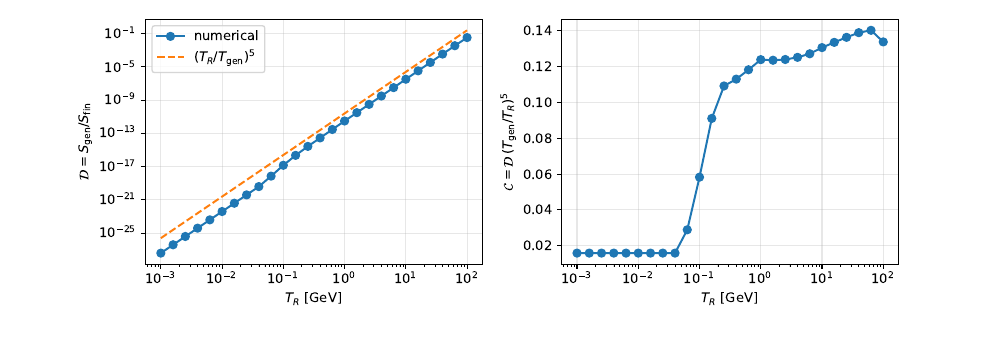
\includegraphics[width=0.9\textwidth]{fig_dilution.png}
\caption{Entropy dilution $\mathcal D=S(T_{\rm gen})/S_{\rm fin}$ for $T_{\rm gen}=131.7$ GeV from Eq.~(\ref{eq:boltz}) (left) and the prefactor $\mathcal C$ (right). The step near $T_R\sim0.1$ GeV is the change of $g_*$ across the QCD crossover in our approximate $g_*(T)$.}
\label{fig:dilution}\end{figure}

\section{Electroweak sphalerons in an EMDE}\label{sec:sph}

\subsection{Susceptibility}
A sphaleron transition changes Chern--Simons number by $\Delta N_{\rm CS}=\pm1$ and produces twelve left-handed doublet fermions. A bias $\mu_{\rm CS}$ conjugate to $N_{\rm CS}$ enforces $n_g(3\mu_Q+\mu_L)=\mu_{\rm CS}$. Imposing Yukawa equilibrium ($\mu_u=\mu_Q+\mu_H$, $\mu_d=\mu_Q-\mu_H$, $\mu_e=\mu_L-\mu_H$), hypercharge neutrality and $B-L=0$, one finds (Appendix~B)
\begin{equation}
n_B=\tfrac{12}{79}T^2\mu_{\rm CS}\quad\Rightarrow\quad Y_B=\xi\,\frac{\mu_{\rm CS}}{T},\qquad \xi=\frac{12/79}{2\pi^2g_*/45}=3.24\times10^{-3}.
\end{equation}
With $\mu_{\rm CS}=0$ the same system gives the standard $B=\tfrac{28}{79}(B-L)$. In an EMDE the Hubble rate at $T\sim150$ GeV is enhanced by $7.9\,T^2/T_R^2$ relative to radiation domination, and the electron Yukawa coupling is out of equilibrium for $T_R\lesssim15$ GeV. Removing $e_R$ from the equilibrium network lowers $\xi$ by $4\%$.

\subsection{Rate and equilibrium window}
The lattice rate for $m_H=125$ GeV is \cite{DRT14}
\begin{equation}
\frac{\Gamma_{\rm sph}}{T^4}=\begin{cases}\exp(0.83\,T/{\rm GeV}-147.7), & 130\ {\rm GeV}<T<T_c,\\ 18\,\alpha_W^5,& T>T_c,\end{cases}\qquad T_c=159\ {\rm GeV}.
\label{eq:rate}
\end{equation}
In radiation domination sphalerons freeze out at $T_*=131.7\pm2.3$ GeV, where the washout rate $\lambda_{\rm sph}=c^{-1}\Gamma_{\rm sph}/T^3$ equals $H$. We fix $c=0.12$ (i.e.\ $1/c\simeq8.5$) to reproduce this value; it is a calibration, not a prediction, and we vary it by a factor of ten below. In an EMDE $H$ is given by Eq.~(\ref{eq:Hss}) and grows as $T^4$, whereas $\Gamma_{\rm sph}/T^3$ grows only as $T$ above $T_c$. Equilibrium therefore holds only in a window
\begin{equation}
T_*(T_R)<T<T_{\rm up}(T_R),\qquad T_{\rm up}^3=\frac{18\,\alpha_W^5\,T_R^2\Mpl}{c\,\kappa}.
\label{eq:window}
\end{equation}
The scaling $T_{\rm up}\propto T_R^{2/3}$ is due to \cite{DLR}; the lattice rate fixes the coefficient and the broken-phase fit fixes the lower edge (Table~\ref{tab:window}). The window closes when $T_{\rm up}=T_c$, i.e.
\begin{equation}
T_R^{\rm eq}=\left(\frac{c\,\kappa\,T_c^3}{18\,\alpha_W^5\Mpl}\right)^{1/2}=2.6\ {\rm MeV}
\end{equation}
(0.8--8.1 MeV for $c\to c/10,\,10c$), at or below the BBN bound. The fit (\ref{eq:rate}) is discontinuous at $T_c$ by a factor $\sim5$, so edges near $T_c$ are uncertain by a few GeV.

\begin{table}[h]\centering
\begin{tabular}{lcccc}\toprule
$T_R$ & 18 MeV & 56 MeV & 1 GeV & 10 GeV\\ \midrule
$T_*$ [GeV] & 156 & 153 & 145 & 139\\
$T_{\rm up}$ [GeV] & 582 & 1296 & $\gtrsim3000$ & $\gtrsim3000$\\ \bottomrule
\end{tabular}
\caption{Sphaleron equilibrium window in an EMDE.}\label{tab:window}\end{table}

\subsection{Washout and conversion efficiencies}\label{sec:boltz}
Let each modulus decay create baryon number $\epsilon_B$ and lepton number $\epsilon_L$. With comoving densities $N_X=n_Xa^3$, $N_\phi=\rho_\phi a^3/m$,
\begin{equation}
\dot N_{B-L}=(\epsilon_B-\epsilon_L)\Gamma N_\phi,\qquad
\dot N_B=\epsilon_B\Gamma N_\phi-\lambda_{\rm sph}(T)\Big(N_B-\tfrac{28}{79}N_{B-L}\Big),
\label{eq:washout}
\end{equation}
to be solved with Eq.~(\ref{eq:boltz}). We use the symmetric-phase target $\tfrac{28}{79}$; the broken-phase correction near freeze-out is a few percent. The system is linear in the sources, so $N_B^{\rm fin}=\eta_B\epsilon_BN_\phi^{\rm tot}$ for $\epsilon_L=0$ and $N_B^{\rm fin}=-\eta_L\epsilon_LN_\phi^{\rm tot}$ for $\epsilon_B=0$, with $\eta_{B,L}$ depending only on $T_R$ (Fig.~\ref{fig:eff}).

\begin{figure}[h]\centering
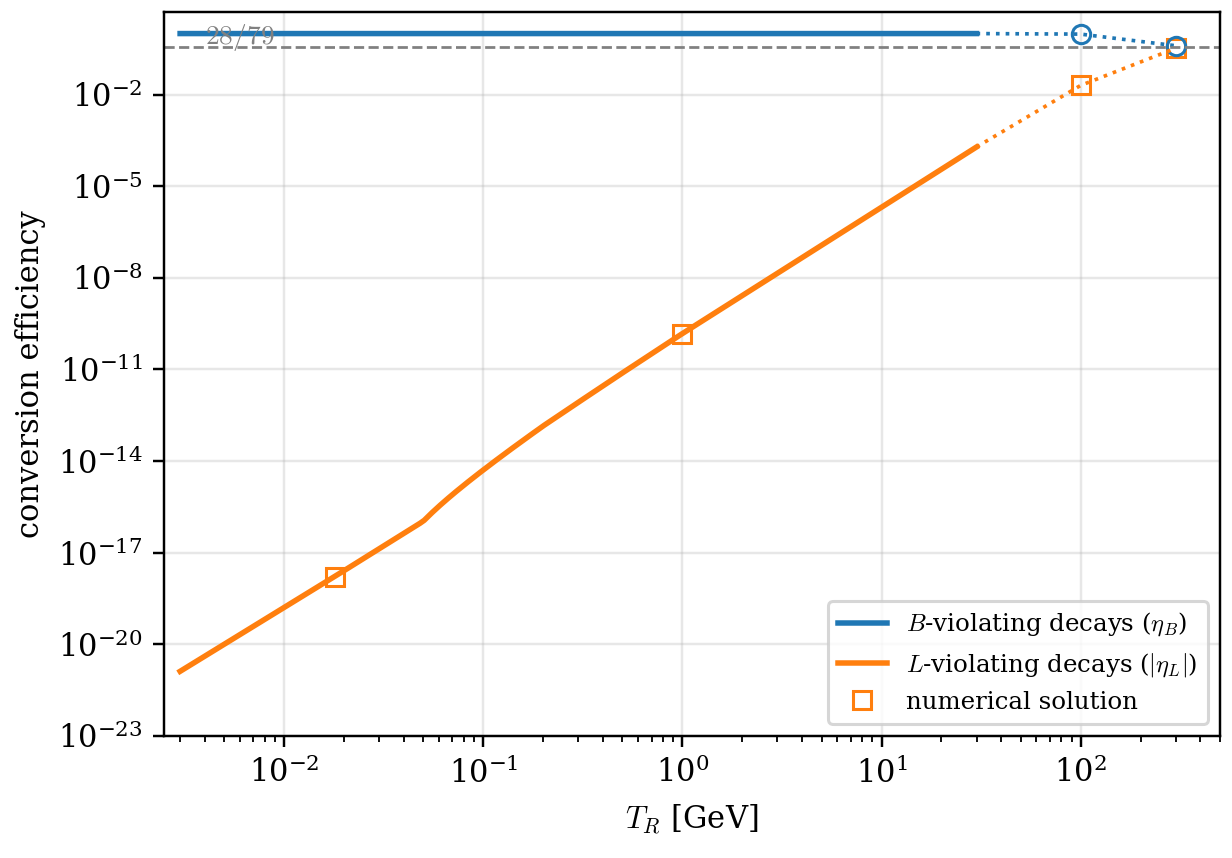
\includegraphics[width=0.62\textwidth]{fig_eff.png}
\caption{Conversion efficiencies. Curves: closed forms (\ref{eq:etaL}) for $T_R\le30$ GeV; open markers: numerical solutions of Eq.~(\ref{eq:washout}); dotted lines join the numerical values at larger $T_R$. Baryon-violating decays survive for $T_R\lesssim30$ GeV; lepton asymmetries are converted only if an appreciable fraction of the decays occurs while sphalerons are in equilibrium.}
\label{fig:eff}\end{figure}

\paragraph*{Closed forms.} For $T_R\ll T_*$ the fraction of the modulus energy that has decayed by $t=2/3H$ is $\Gamma t=\tfrac23\Gamma/H$. Lepton number produced before sphaleron freeze-out is converted with coefficient $28/79$, and all later decays leave $B$ untouched. Using Eqs.~(\ref{eq:TR}) and (\ref{eq:Hss}), $\Gamma/H=\tfrac{2g_R}{5g_*}(T_R/T)^4$, so
\begin{equation}
\eta_L\simeq\frac{28}{79}\cdot\frac23\frac{\Gamma}{H(T_*)}=\frac{28}{79}\,\frac{4}{15}\,\frac{g_R}{g_*}\left(\frac{T_R}{T_*}\right)^4,\qquad
\eta_B\simeq1-\frac{51}{79}\cdot\frac23\frac{\Gamma}{H(T_*)}.
\label{eq:etaL}
\end{equation}
Here $T_*=T_*(T_R)$ is the lower edge of the window from Table~\ref{tab:window}; with it, Eq.~(\ref{eq:etaL}) gives $1.7\times10^{-18}$, $1.5\times10^{-10}$, $2.0\times10^{-6}$ at $T_R=18$ MeV, 1 GeV, 10 GeV, within $10\%$ of the numerical solution. (Using the radiation-domination value $T_*=131.7$ GeV overestimates $\eta_L$ by up to a factor 2.) Numerically $\eta_B=1$ to better than $10^{-3}$ for $T_R\lesssim30$ GeV, falling to $0.96$ at 100 GeV and $0.40$ at 300 GeV; $\eta_L\simeq1.4\times10^{-10}(T_R/{\rm GeV})^{4.1}$ for 1--10 GeV, reaching $0.02$ at 100 GeV and $0.33$ at 300 GeV. Leptogenesis from modulus decay therefore needs $T_R\gtrsim100$--$300$ GeV; for $T_R\lesssim30$ GeV the sphalerons are spectators. Multiplying Eq.~(\ref{eq:etaL}) by the decay yield $\epsilon\kappa_YT_R/m$ gives $Y_B\propto\epsilon\,T_R^5/(T_*^4m)$, the scaling found for non-thermal leptogenesis in \cite{Garcia}.

\section{Axion-driven sources}\label{sec:axion}

Let $\theta^i=a^i/f$ have kinetic term $\tfrac12G_{ij}\dot\theta^i\dot\theta^j$ and couple through $\mathcal L\supset\frac{g^2}{32\pi^2}c_i\theta^iW\tilde W$ with constant $c_i$. In string compactifications $c_i=k_i$ are the integers in $f_W=k_iT^i$. Since $\frac{g^2}{32\pi^2}W\tilde W=\partial_\mu K^\mu$,
\begin{equation}
\mu_{\rm CS}=\frac{d}{dt}(c_i\theta^i)=c_i\dot\theta^i.
\end{equation}
\emph{Remark (frame independence).} $c_i\theta^i$ is a scalar, so $\mu_{\rm CS}$ is unchanged by any time-dependent rotation $R(t)$ of the field-space basis: $\tilde c_\alpha\dot{\tilde\theta}^\alpha+\dot{\tilde c}_\alpha\tilde\theta^\alpha=c_i\dot\theta^i$. In particular a rotating eigenbasis, such as an avoided crossing in a thermal mass matrix, produces no chemical potential unless the axions acquire a coordinate velocity.

Define $F\equiv(c_iG^{ij}c_j)^{-1/2}$; for one axion with $\theta=a/f$, $F=f/N$.

\paragraph*{Bound.} If sphalerons are in equilibrium at $T_{\rm gen}$ and $\rho_{\rm kin}=\tfrac12G_{ij}\dot\theta^i\dot\theta^j\le\rho_{\rm tot}=3H^2\Mpl^2$, the Cauchy--Schwarz inequality in the metric $G$ gives $|c_i\dot\theta^i|\le F^{-1}\sqrt{2\rho_{\rm kin}}$, hence
\begin{equation}
Y_B^{\rm gen}\le\xi\,\frac{\sqrt6\,H(T_{\rm gen})\Mpl}{F\,T_{\rm gen}}
\;\xrightarrow{\rm RD}\;\xi\,\pi\sqrt{\frac{g_*}{15}}\frac{T_{\rm gen}}{F}\simeq\frac{3.6\ {\rm GeV}}{F},\qquad
F\le F_{\max}=4.2\times10^{10}\ {\rm GeV}.
\label{eq:Fmax}
\end{equation}
Only the sphaleron freeze-out region contributes, because $B+L$ relaxes to its equilibrium value while sphalerons are active and $B-L$ is not generated by $\mu_{\rm CS}$; thus $T_{\rm gen}=T_*(T_R)$. The bound uses no information about the source and is saturated only if the axion kinetic energy equals the total energy density (kination). In an EMDE, $Y_B^{\rm fin}\propto H_{\rm EMDE}\mathcal D\propto T_R^{3}$, so an EMDE only weakens the mechanism: for $T_R\le30$ GeV the maximal yield is lower by $4.9\times10^{-3}$, $F_{\max}\to2\times10^8$ GeV. A source limited by the Hubble rate, $|c_i\dot\theta^i|\le\nu H$, gives $Y_B\le\xi\nu H/T$, which at $T=131.7$ GeV requires $\nu\gtrsim10^8$.

For a single axion, with $n_\theta=f^2\dot\theta$ and $Y_\theta=n_\theta/s$, the same susceptibility gives $Y_B=\tfrac{12}{79}N(T^2/f^2)Y_\theta$, the relation underlying axiogenesis \cite{CoHarigaya}.

\paragraph*{Dark-matter-constrained version.} If the rotation ends as cold axion dark matter with conserved PQ charge, $m_aY_\theta^{\rm fin}\le\rho_{\rm DM}/s=4.4\times10^{-10}$ GeV. Baryons and axions are diluted equally, so for any EMDE history
\begin{equation}
\frac{f^2m_a}{N}\le\frac{(12/79)\,T_{\rm gen}^2(\rho_{\rm DM}/s)}{Y_B^{\rm obs}}=1.35\times10^4\ {\rm GeV}^3.
\end{equation}
For the QCD axion, $m_af\simeq5.7\times10^{-3}$ GeV$^2$ gives $f\lesssim2\times10^6N$ GeV. This is more restrictive than the values $10^7$--$10^8$ GeV quoted in the axiogenesis literature. The bound can be evaded by dissipating the rotation \cite{Asadi}, which is why Eq.~(\ref{eq:Fmax}), which assumes nothing about the endpoint, is the more robust statement.

\paragraph*{Classification.} Let $H_*=H(T_*)$. (A) $m_a\lesssim H_*$: the field is frozen, $|\dot\theta|\lesssim H_*\theta$, and the Hubble-limited bound applies. (B) $m_a\gg H_*$, $\Gamma_a\ll H_*$: the axion oscillates and is long lived; Eq.~(\ref{eq:Fmax}) applies. (C) $\Gamma_a\gtrsim H_*$: the oscillation is suppressed by $e^{-\Gamma_a/4H_*}$ and no coherent velocity survives at freeze-out.

\section{Generic bound on $T_R$ for pre-decay generation}\label{sec:generic}

Let a mechanism act at $T_{\rm gen}$ with maximal chemical potential $(\mu/T)_{\max}$. Then $Y_B^{\rm fin}\le\mathcal D(T_R)\,\xi\,(\mu/T)_{\max}$, and
\begin{equation}
T_R\ge T_R^{\min}\simeq T_{\rm gen}\left[\frac{Y_B^{\rm obs}}{\mathcal C\,\xi\,(\mu/T)_{\max}}\right]^{1/5}.
\end{equation}
For $T_{\rm gen}=131.7$ GeV: $T_R^{\min}=6.1,\,9.6,\,15.1,\,23.9,\,37.7$ GeV for $(\mu/T)_{\max}=1,\,10^{-1},\dots,10^{-4}$. Since $T_R^{\min}\propto T_{\rm gen}$, mechanisms operating at lower temperature are less constrained; the bound applies to generation at the electroweak scale or above. In terms of the modulus mass, with $\Gamma=c_\Gamma m^3/4\pi\Mpl^2$ and $c_\Gamma=1$, $T_R\ge6.1$ GeV is $m_\Phi\gtrsim1.5\times10^7$ GeV (scaling as $c_\Gamma^{-1/3}$), about two orders of magnitude above the value $m_\Phi\gtrsim1.2\times10^5$ GeV required by BBN.

\section{Application to the Large Volume Scenario}\label{sec:lvs}

\subsection{Explicit vacua}
We use the Swiss-cheese compactification on $\mathbb P^4_{[1,1,1,6,9]}$ ($h^{1,1}=2$, $\chi=-540$) \cite{BBCQ}, with
\begin{equation}
K=-2\ln\!\big(\mathcal V+\tfrac{\hat\xi}{2}\big),\quad\mathcal V=\gamma(\tau_b^{3/2}-\tau_s^{3/2}),\quad W=W_0+Ae^{-aT_s},
\end{equation}
$\gamma=1/9\sqrt2$, $\hat\xi=-\zeta(3)\chi/2(2\pi)^3g_s^{3/2}$, $W_0=|A|=1$, $g_s=0.3$ ($0.4$ for the smallest volumes), $a=2\pi/N$ treated as continuous. The exact $\mathcal N=1$ potential is minimised at high precision and the Hessian checked to be positive definite. The vacua are AdS, which changes masses at $O(1)$ relative to a de Sitter vacuum. Ten vacua cover $\vol=2.5\times10^3$--$10^{16}$. They confirm $m_{3/2}\simeq\Mpl/\vol$, $m_{\tau_b}=c_m\Mpl\vol^{-3/2}$ with $c_m=1.0$--$2.1$, and $m_{\tau_s}\simeq m_\rho\simeq(17$--$78)\,m_{3/2}$; a modulus mass of $10^5$ GeV corresponds to $\vol\sim10^9$, not $10^{15}$. We take $\Gamma=c_\Gamma m^3/4\pi\Mpl^2$ with $c_\Gamma=1$ (varied between 0.3 and 8). The width to the bulk axion partner, $m^3/48\pi\Mpl^2$ \cite{CCQ}, produces dark radiation; $\Delta N_{\rm eff}<0.3$ requires $c_\Gamma\gtrsim0.9$--$1.8$ \cite{HT}.

For the K3-fibred model \cite{CBQ} the fibre modulus is the lightest. With the string-loop potential of \cite{CBQ}, which is conjectural, we find $m_f=c_f\Mpl\vol^{-5/3}$ with $c_f=1.45$ for the reference loop data (0.70--3.0 under factor-of-three variations; 17 for the published TeV-scale parameter set), so $T_R\propto\Mpl\vol^{-5/2}$. For the published LV set the numerical fibre mass reproduces the analytic $m_f^2=4(1+\tfrac76R)C_2^2/\vol^{10/3}$ to fourteen digits. If heavier moduli decay earlier, additional dilution can only reduce the final asymmetry, so the bounds below hold for multi-stage histories.

\begin{table}[h]\centering
\begin{tabular}{lccc}\toprule
Maximal $\vol$ for & $T_R\ge6.1$ GeV & $T_R\ge100$ GeV & $T_R\ge4$ MeV\\ \midrule
Swiss-cheese & $3.8\times10^7$ & $1.1\times10^7$ & $1.2\times10^9$\\
K3-fibred, $c_f=1.45$ & $6.6\times10^6$ & $2.1\times10^6$ & $1.5\times10^8$\\
K3-fibred, $c_f=0.7$--$3.0$ & $4.3\times10^6$--$1.0\times10^7$ & $1.4\times10^6$--$3.3\times10^6$ & $9.8\times10^7$--$2.4\times10^8$\\ \bottomrule
\end{tabular}
\caption{Upper bounds on $\vol$ from pre-decay electroweak baryogenesis, decay leptogenesis, and BBN.}\label{tab:vol}\end{table}

\subsection{Channel by channel}
\emph{Pre-decay electroweak baryogenesis} requires $T_R\gtrsim6$--$38$ GeV, i.e.\ $\vol\lesssim3.8\times10^7$ (Swiss-cheese) and $7\times10^6$ (K3), $m_{3/2}\gtrsim10^{10}$ GeV. At $\vol=10^{16}$, $T_R\simeq6\times10^{-19}$ GeV.

\emph{Axion-driven baryogenesis.} For $f_W=NT$ with $T$ a bulk or fibre modulus, $K_{T\bar T}=O(1)/\tau^2$ and $\alpha_W^{-1}=N\tau$, so
\begin{equation}
F=\frac{\kappa_F\,\alpha_W\Mpl}{4\pi},\qquad\kappa_F=2\tau\sqrt{2K_{T\bar T}}=O(1)\ (\sqrt2\ \text{for the fibre}),
\end{equation}
independent of $N$ and $\tau$: $F\simeq9.3\times10^{15}$ GeV, $2\times10^5$ times the bound (\ref{eq:Fmax}), even at kination. For the Standard Model on a blow-up cycle, $K_{s\bar s}\simeq3\gamma/8\sqrt{\tau_s}\vol$ and $F_s\simeq4.0\times10^{16}\,{\rm GeV}/\sqrt{\vol}$, which satisfies (\ref{eq:Fmax}) for $\vol\gtrsim9\times10^{11}$. But the axion is heavy, $m_\rho\simeq(17$--$78)m_{3/2}$, and decays to gauge bosons with $\Gamma_\rho\simeq\tfrac38\alpha_W^2m_\rho^3/32\pi^3F_s^2$; in the explicit vacua $\Gamma_\rho/H(T_*)\ge2.3\times10^3$ for all $\vol$, so it is of type (C) and provides no velocity. (For $\vol\gtrsim10^{10}$ the radiation at $T_*$ is not in the steady state, but there $T_R$ is far below BBN in any case.)

\emph{Lepton-violating decays.} $\eta_L\simeq1.4\times10^{-10}(T_R/{\rm GeV})^{4.1}$, so $T_R\gtrsim100$ GeV is needed: $\vol\lesssim1.1\times10^7$.

\emph{Baryon-violating decays.} With $\epsilon$ the CP-violating baryon number per decay, $Y_B=\epsilon\,\eta_B\kappa_YT_R/m$ with $\kappa_Y\simeq0.7$--$0.9$. Since $T_R/m\propto\vol^{-3/4}$, $\vol_{\max}\propto\epsilon^{4/3}$; in the explicit vacua $\vol_{\max}=3.1\times10^{12},\,7.3\times10^9,\,2.6\times10^6,\,6.5\times10^3$ for $\epsilon=1,\,10^{-2},\,10^{-4},\,10^{-6}$. TeV-scale LVS requires $\epsilon\gg1$. The value of $\epsilon$ is model dependent; mechanisms in which it is fixed, through the decay chain modulus $\to$ gaugino pair $\to$ $udd$, are described in \cite{IJT,KW} for KKLT-type and other stabilisation schemes; the LVS case is considered next.


\subsection{Sequestered soft terms and the required CP asymmetry}\label{sec:seq}
In sequestered LVS the soft terms on the Standard Model brane are suppressed relative to $m_{3/2}\sim\Mpl/\vol$ by at least $\vol^{-1/2}$ and may be as small as $\Mpl/\vol^2$; gaugino masses are of order $m_{3/2}/\vol$, and scalar masses are either comparably small or larger by $\vol^{1/2}$ \cite{BCKMQ}. For TeV soft terms \cite{BCKMQ} quotes $\vol\sim10^{6}$--$10^{7}$; the precise value depends on $W_0$ and $g_s$. For the vacua used here ($W_0=1$), $m_{\rm soft}=\Mpl/\vol^2$ lies between 10 TeV and 0.1 TeV for $1.5\times10^7\lesssim\vol\lesssim1.5\times10^8$. In this range $m_{3/2}\sim10^{10}$--$10^{11}$ GeV, $m_{\tau_b}\simeq2\times10^6$--$6\times10^7$ GeV and $T_R\simeq0.4$--$50$ GeV, so that $\eta_B\simeq1$ (Sec.~\ref{sec:boltz}), and decays to superpartners are kinematically open. Solving $Y_B=\epsilon\,\eta_B\kappa_YT_R/m$ for $\epsilon$ gives (Fig.~\ref{fig:eps})
\begin{equation}
\epsilon\simeq1.3\times10^{-4},\ 2.8\times10^{-4},\ 5.6\times10^{-4}\qquad\text{at }\vol=1.5\times10^7,\ 5\times10^7,\ 1.5\times10^8,
\end{equation}
with a minimum $\epsilon\simeq2\times10^{-4}$ near $\vol=3\times10^7$.

This requirement is to be compared with what the decay chain can supply. In the mechanism of \cite{KW} the modulus decays to a gaugino pair, and the gluino decays to $tsb$ through $W\supset\lambda''_{323}U^cD^cD^c$ with a CP asymmetry from the interference of tree and loop diagrams; in our normalisation $\epsilon=\tfrac43\,\mathrm{Br}\,\epsilon_{\rm CP}$, with $\epsilon_{\rm CP}\lesssim3\times10^{-4}\sin2\phi_{12}$ for the MSSM spectra of \cite{KW}. The branching ratios follow from the supergravity data. We have computed them in the vacua of Sec.~\ref{sec:lvs} using the decay widths of \cite{KW}, with the light eigenstate $\Phi$ of $G^{-1}\partial^2V$ normalised canonically and $\delta\tau^i=v^i\phi$. The width to the massless axion of $T_b$ is
\begin{equation}
\Gamma_{aa}=\frac{g^2m^3}{128\pi\Mpl^2},\qquad g=\frac{\partial_\phi K_{b\bar b}}{K_{b\bar b}},\qquad g^2=\frac83,
\end{equation}
that is $\Gamma_{aa}=m^3/48\pi\Mpl^2$, which we confirm numerically to four digits in each vacuum. For the Higgs sector, with $Z\propto\vol^{-2/3}$ one finds $\partial_\phi\ln Z=\sqrt{2/3}$ in every vacuum, so that
\begin{equation}
\Gamma_{HH}=\Gamma_{\tilde h\tilde h}=2z^2\,\Gamma_{aa},\qquad z\equiv Z/\hat Z,
\end{equation}
and $\mathrm{Br}_{\tilde h\tilde h}=2z^2/(1+4z^2+\Gamma_{gg}/\Gamma_{aa})$, which is $0.40$ for $z=1$ and $0.25$ for $z=1/2$. For gauge bosons and gauginos two cases arise. If the gauge kinetic function is $f=T_s$, as for a stack wrapping the blow-up cycle, then $\Gamma_{gg}/\Gamma_{aa}=0.03$--$0.06$ (Table~\ref{tab:br}) and the gaugino mass $M_{\tilde\lambda}=F^{T_s}/2\tau_s$ exceeds $m_\Phi$ by a factor $17$--$630$, which grows as $\vol^{1/2}$; the gaugino-pair channel is closed. If $f$ does not depend on $T_b$ or $T_s$, as for D3-branes at a singularity at leading order, then $\partial_\Phi f=0$ and $\Gamma_{gg}$ and $\Gamma_{\tilde\lambda\tilde\lambda}$ vanish at tree level; the sequestered gaugino masses of order $m_{3/2}/\vol$ lie below $m_\Phi$, but the corresponding couplings arise only at loop level and from anomaly-mediated terms, which are further suppressed. In neither case is $\mathrm{Br}_{\tilde\lambda\tilde\lambda}$ of order one, so the gluino chain of \cite{KW} does not operate in LVS.

\begin{table}[h]\centering
\begin{tabular}{rcccc}\toprule
$\vol$ & $m_\Phi$ [GeV] & $M_{\tilde\lambda}/m_\Phi$ ($f=T_s$) & $\Gamma_{gg}/\Gamma_{aa}$ ($f=T_s$) & $(\Gamma_{HH}+\Gamma_{\tilde h\tilde h})/\Gamma_{aa}$\\ \midrule
$2.6\times10^{5}$ & $3.0\times10^{10}$ & 17 & 0.063 & $4z^2$\\
$3.4\times10^{6}$ & $6.0\times10^{8}$ & 54 & 0.045 & $4z^2$\\
$1.2\times10^{7}$ & $8.3\times10^{7}$ & 99 & 0.039 & $4z^2$\\
$4.5\times10^{7}$ & $1.1\times10^{7}$ & 183 & 0.034 & $4z^2$\\
$1.7\times10^{8}$ & $1.6\times10^{6}$ & 339 & 0.029 & $4z^2$\\
$6.1\times10^{8}$ & $2.1\times10^{5}$ & 630 & 0.026 & $4z^2$\\ \bottomrule
\end{tabular}
\caption{Light-modulus decay widths in the explicit Swiss-cheese vacua ($W_0=A=1$, $g_s=0.3$, no uplift), from the formulas of \cite{KW} with $N_g=12$.}\label{tab:br}\end{table}

The baryon asymmetry must then be carried by the Higgs sector. In the pattern of the hidden-gaugino variant of \cite{KW}, in which a fermion decays through a gluino loop with $\epsilon_{\rm CP}$ up to $10^{-2}$, a higgsino pair with $\mathrm{Br}_{\tilde h\tilde h}\lesssim0.4$ requires $\epsilon_{\rm CP}\simeq(1.6$--$7)\times10^{-4}$ across the window. We have computed this asymmetry by an explicit amplitude calculation (Appendix~\ref{app:amp}). The neutral higgsino couples to the top and the stop through $W\supset y_tH_uQU^c$, with the structures $(\tilde h\psi_Q)\tilde t_R^*$ and $(\tilde h\psi_{U^c})\tilde t_L$, each with coefficient $y_t/\sqrt2$ for a Majorana mass eigenstate; unlike the gluino, it couples the top of one chirality to the stop of the other. With the stops integrated out, the amplitudes are governed by the propagator matrix $D=(M^2_{\tilde t})^{-1}$ in the $(\tilde t_R,\tilde t_L)$ basis. The absorptive part comes from the cut through $\tilde g\,\bar t$, and the CP-odd term is proportional to $m_{\tilde h}m_{\tilde g}f_2(m_{\tilde g}^2/m_{\tilde h}^2)\sin\phi_{12}$, where $\phi_{12}$ is the relative phase of the two Majorana masses. The two coupling structures contribute to this term with equal magnitude and opposite sign: a gaugino mass insertion enters with the phase $e^{i\phi}$ for a coupling to $\lambda\psi$ and $e^{-i\phi}$ for a coupling to $\lambda^\dagger\psi^\dagger$. For a pure higgsino they cancel. The asymmetry vanishes at this order for any stop masses, any stop mixing and any phase of $X_t$; we find $|\epsilon_{\rm CP}|<10^{-18}$ over a scan of these parameters. A bino admixture $a_B$ breaks the symmetry between the structures and gives
\begin{equation}
\epsilon_{\rm CP}\simeq7\times10^{-4}\,a_B\qquad(m_{\tilde t}=2\mu,\ X_t=2.5\,m_{\tilde t},\ m_{\tilde g}=0.4\mu,\ \sin\phi_{12}=1,\ \lambda''\gg g_3),
\end{equation}
which reaches the required $(1.6$--$7)\times10^{-4}$ for $a_B\gtrsim0.25$ (Fig.~\ref{fig:higgsino}); for $m_{\tilde t}=3\mu$ it requires $a_B\gtrsim0.6$. The higgsino chain therefore generates the required asymmetry only for a well-tempered bino--higgsino state ($M_1\simeq\mu$) with stops within a factor two or three of the higgsino mass, and $\mu>m_{\tilde g}$.

\begin{figure}[h]\centering
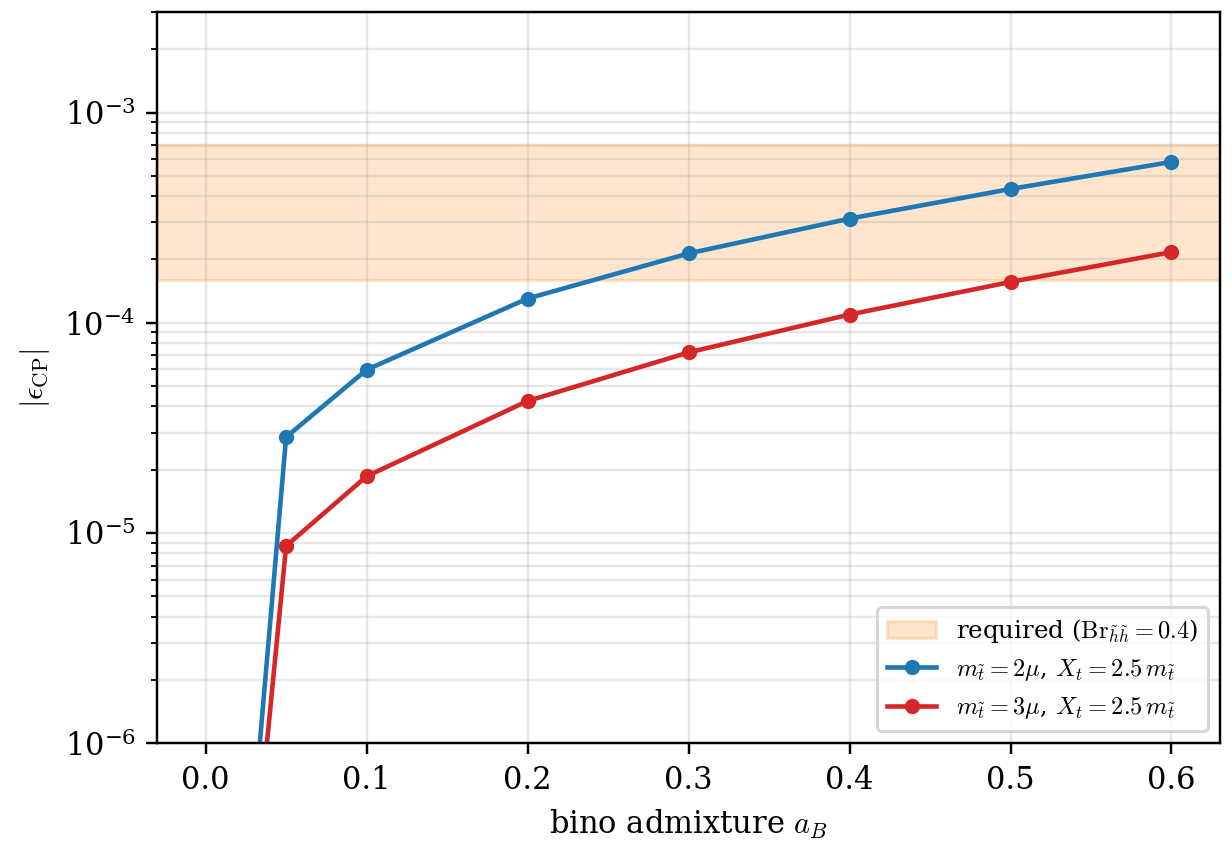
\includegraphics[width=0.62\textwidth]{fig_higgsino.png}
\caption{CP asymmetry in the decay of a neutralino, a mixture of the neutral higgsino and the bino with bino fraction $a_B$, to $tsb$ through a gluino loop ($\sin\phi_{12}=1$, $m_{\tilde g}=0.4\mu$). The asymmetry vanishes for $a_B=0$. The band is the asymmetry required in sequestered LVS for $\mathrm{Br}_{\tilde h\tilde h}=0.4$.}
\label{fig:higgsino}\end{figure}
\begin{figure}[h]\centering
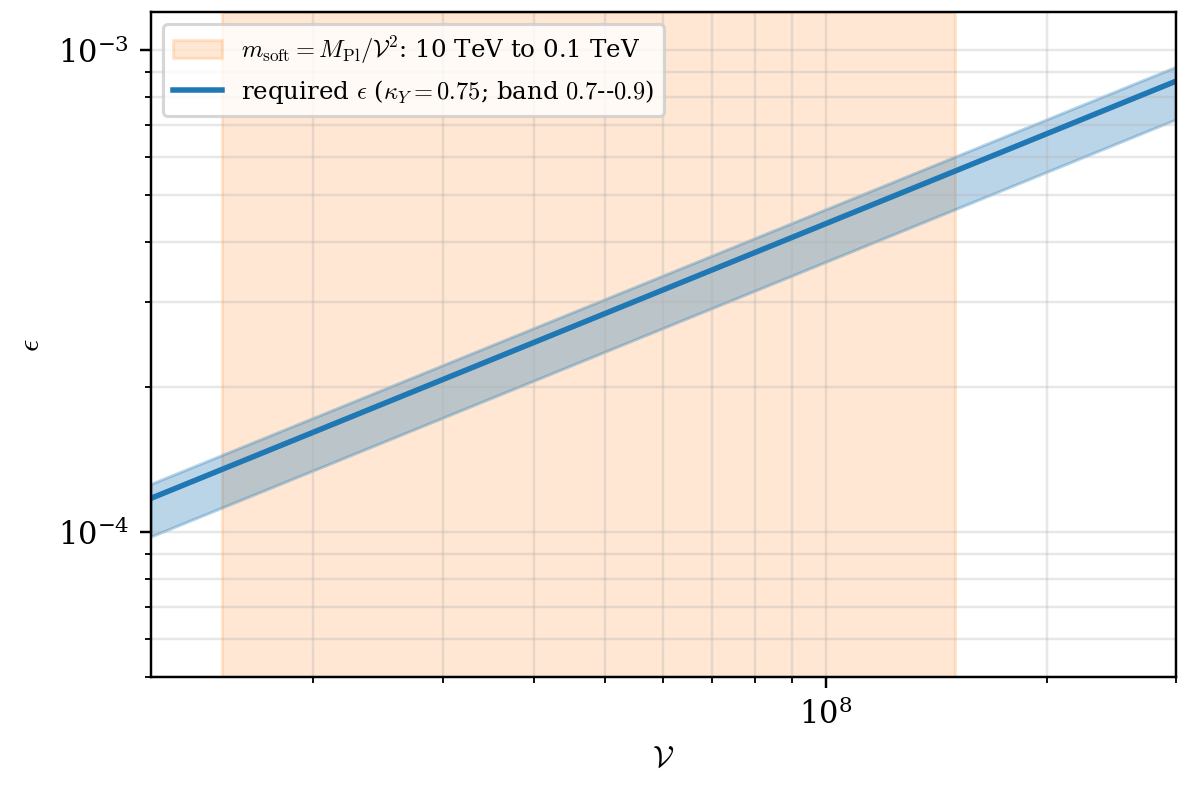
\includegraphics[width=0.62\textwidth]{fig_eps.png}
\caption{CP-violating baryon number per decay required to reproduce $Y_B^{\rm obs}$ from baryon-violating decays of the volume modulus in the explicit Swiss-cheese vacua, for $T_R\lesssim100$ GeV where $\eta_B\simeq1$.}
\label{fig:eps}\end{figure}

\subsection{Other moduli stabilisation schemes}\label{sec:cross}
The entropy wall does not depend on the construction, only on $m_\Phi$ and the total width. Table~\ref{tab:cross} applies Eqs.~(\ref{eq:D}) and (\ref{eq:etaL}) to the three classes of compactification studied in \cite{KW}, using the decay coefficients $\Gamma=c\,m^3/\Mpl^2$ listed there (IIB/KKLT: $c_{\rm tot}\simeq0.13$, $m_\Phi=10^6$--$8\times10^6$ GeV; heterotic: $c_{\rm tot}\simeq0.21$, $m_\Phi=2$--$6\times10^6$ GeV; $G_2$: $0.1\le c_{\rm tot}\le36$, $m_\Phi=6\times10^4$--$1.6\times10^5$ GeV), together with the sequestered LVS window of Sec.~\ref{sec:seq}.

\begin{table}[h]\centering\small\setlength{\tabcolsep}{4pt}
\begin{tabular}{lccccc}\toprule
 & $T_R$ [GeV] & $\mathcal D(131.7\ {\rm GeV})$ & $\eta_L$ & $\epsilon_{\rm req}$ & gaugino pairs\\ \midrule
IIB / KKLT & 0.16--3.0 & $10^{-16}$--$10^{-9}$ & $10^{-14}$--$10^{-8}$ & $(3$--$7)\times10^{-4}$ & open\\
heterotic & 0.5--2.5 & $10^{-13}$--$10^{-10}$ & $10^{-11}$--$10^{-8}$ & $(2.7$--$4.5)\times10^{-4}$ & open\\
$G_2$ & 0.003--0.17 & $10^{-26}$--$10^{-16}$ & $10^{-21}$--$10^{-13}$ & $(1$--$24)\times10^{-4}$ & open\\
sequestered LVS & 0.4--54 & $10^{-14}$--$10^{-3}$ & $10^{-10}$--$0.02$ & $(1.3$--$5.6)\times10^{-4}$ & closed\\ \bottomrule
\end{tabular}
\caption{Entropy-wall quantities in four moduli-dominated cosmologies. $\epsilon_{\rm req}=Y_B^{\rm obs}/Y_\Phi$ with $Y_\Phi=\tfrac34T_R/m_\Phi$ is the baryon number per modulus decay required of baryon-violating decays. The last column states whether the modulus can decay to a gaugino pair: open in \cite{KW} for the first three, closed in LVS (Sec.~\ref{sec:seq}).}\label{tab:cross}\end{table}

In every case $T_R$ lies below the $6.1$ GeV required for electroweak-scale generation before the decay, which in these schemes translates into $m_\Phi\gtrsim1.1$--$1.4\times10^7$ GeV for $c_{\rm tot}\lesssim0.2$ and $2\times10^6$ GeV for $c_{\rm tot}=36$. A pre-decay asymmetry is therefore diluted by $10^{-9}$--$10^{-26}$, and lepton-violating decays are converted with $\eta_L\lesssim10^{-8}$ except in the upper part of the LVS window. What survives is baryon-violating decay, and the required baryon number per decay, $\epsilon_{\rm req}\sim10^{-4}$--$10^{-3}$, is the same in all four constructions. It is a property of the entropy wall, not of the stabilisation scheme. LVS differs in whether the decay chain that would supply $\epsilon$ exists: the gaugino-pair channel used in \cite{KW} is open for the first three and closed for LVS.


\begin{table}[h]\centering\small
\begin{tabular}{p{4.0cm}p{5.6cm}p{4.9cm}}\toprule
Channel & Condition & $\vol$ range\\ \midrule
Pre-decay EW baryogenesis & $T_R\gtrsim6$--$38$ GeV & $\lesssim(1.7$--$3.8)\times10^7$\\
Axion velocity, bulk/fibre & $F\lesssim4\times10^{10}$ GeV & excluded ($F\simeq9\times10^{15}$)\\
Axion velocity, blow-up & $\Gamma_\rho\gtrsim H_*$ & excluded (fast decay)\\
Decay leptogenesis & $T_R\gtrsim100$--$300$ GeV & $\lesssim1.1\times10^7$\\
$B$-violating decays & $\epsilon\,\eta_B\kappa_YT_R/m\simeq Y_B^{\rm obs}$ & $\lesssim3.1\times10^{12}\epsilon^{4/3}$\\
$B$-violating decays, sequestered & $\epsilon\simeq(1$--$6)\times10^{-4}$; gluino chain closed & $1.5\times10^7$--$1.5\times10^8$\\
Affleck--Dine, baryonic & see Sec.~\ref{sec:ad} & $\lesssim6\times10^5\,\zeta$; $\lesssim10^4$ in the effective theory\\ \bottomrule
\end{tabular}
\caption{Summary of constraints on LVS, assuming a single modulus-dominated era and no thermal inflation.}\label{tab:sum}\end{table}

\section{Affleck--Dine baryogenesis}\label{sec:ad}

\subsection{Setup}
For a flat direction lifted by $W=\lambda\phi^n/(nM_*^{n-3})$,
\begin{equation}
V=(m_{\rm AD}^2-cH^2)|\phi|^2+\frac{\lambda^2|\phi|^{2n-2}}{M_*^{2n-6}}+\Big(\frac{(a\,m_{\rm AD}e^{i\alpha}+a_HHe^{i\alpha_H})\lambda\phi^n}{nM_*^{n-3}}+{\rm h.c.}\Big).
\label{eq:ADV}
\end{equation}
For $H\gg m_{\rm AD}$ the field tracks $|\phi_0|^2=\big(\sqrt{c/(n-1)}\,HM_*^{n-3}/\lambda\big)^{2/(n-2)}$ and begins to oscillate at $H=m_{\rm AD}$, leaving a charge density $n_B=\epsilon\,m_{\rm AD}|\phi_0|^2$. The relative phase $\delta=\alpha-\alpha_H$ is the CP-violating input. The $udd$ direction has $n=6$; $LH_u$ has $n=4$. The operator scale $M_*$ is not fixed by the four-dimensional analysis; we write $M_*=\zeta\Mpl$. Sec.~\ref{sec:eft} shows that the result depends sharply on $\zeta$.

\subsection{Yield}
We consider $m_{\rm AD}>m_{\rm mod}$, the generic LVS ordering ($m_{\rm AD}\sim m_{3/2}$, $m_{\rm mod}/m_{3/2}\sim\vol^{-1/2}$), with inflaton oscillations until $H\simeq m_{\rm AD}$ and reheating at $T_{\rm RH}\le T_{\rm AD}$, $3m_{\rm AD}^2\Mpl^2=\tfrac{\pi^2}{30}g_*T_{\rm AD}^4$. The maximal yield is $Y_{\rm AD}=\epsilon|\phi_0|^2T_{\rm AD}/4m_{\rm AD}\Mpl^2$; for lower $T_{\rm RH}$ it is reduced by $T_{\rm RH}/T_{\rm AD}$, so what follows are upper bounds. The modulus later oscillates at $H=m_{\rm mod}$ with energy fraction $r_i=\Delta^2/6\Mpl^2$ and produces the dilution $\mathcal D=\tfrac43\kappa_Y(T_R/T_i)(1-r_i)/r_i$, $T_i\propto\sqrt{m_{\rm mod}\Mpl}$. For $n=6$ the dependence on $m_{\rm AD}$ cancels, and
\begin{equation}
Y_B\simeq0.13\,\eta\,\epsilon\,\zeta^{3/2}\sqrt{c_\Gamma}\,\frac{m_{\rm mod}}{\Mpl}\qquad(r_i=\tfrac16,\ c=\lambda=1,\ g_*=106.75).
\label{eq:YAD}
\end{equation}
The coefficient is $0.24$ for $g_R=10.75$; the dependence on $c$ and $\lambda$ is weak ($c^{1/4}\lambda^{-1/2}$), while $Y_B\propto1/r_i$, so $\Delta=\Mpl$ is the conservative choice. Because $T_R\gg T_*$ in the relevant range, $\eta=28/79$ for both baryonic and leptonic directions. For $\zeta=1$, $\epsilon=0.51$, $Y_B=Y_B^{\rm obs}$ requires $m_{\rm mod}\gtrsim8.7\times10^9$ GeV.

\subsection{Charge efficiency}
We integrate the field equations of (\ref{eq:ADV}) in a matter-dominated background ($H=2/3t$) in units $\phi=\Mpl f$, $\tau=m_{\rm AD}t$, $h=H/m_{\rm AD}$. For $h\gg1$ the equations have a scale-free attractor $f=R\,t^{-1/(n-2)}e^{i\theta_{\min}}$ with $n\theta_{\min}+\arg a_{\rm tot}=\pi$; starting on it with the exact velocity removes transients that otherwise change $\epsilon$ by a factor two. The comoving charge is normalised to $a^3m_{\rm AD}|\phi_0|^2$ at $H=m_{\rm AD}$, which defines $\epsilon$. For the benchmark $a=a_H=c=\lambda=1$, $\delta=\pi/2$ we find $|\epsilon|=0.51$ ($n=6$) and $0.69$ ($n=4$). A scan of 162 points ($c,a,a_H\in\{0.3,1,3\}$, six values of $\delta$) gives median $|\epsilon|=0.16$, 90th percentile $0.55$, maximum $1.2$. The benchmark has maximal CP phase; the median is the more representative value.

\subsection{Results for $M_*=\Mpl$}
For $m_{\rm AD}=0.1\,m_{3/2}$, $r_i=\tfrac16$, $c_\Gamma=1$, the maximal volume for which $Y_B^{\rm obs}$ is reached is, for $\epsilon=1.2,\,0.51,\,0.16$:
\begin{center}\begin{tabular}{lccc}\toprule
 & $\epsilon=1.2$ & $0.51$ & $0.16$\\ \midrule
$udd$, Swiss-cheese & $1.1\times10^6$ & $5.9\times10^5$ & $2.8\times10^5$\\
$udd$, K3-fibred & $2.5\times10^5$ & $1.5\times10^5$ & $7.3\times10^4$\\
$LH_u$, Swiss-cheese & $1.9\times10^4$ & $1.2\times10^4$ & $6.9\times10^3$\\ \bottomrule
\end{tabular}\end{center}
At $\vol=5.9\times10^5$, $m_{3/2}=4.1\times10^{12}$ GeV, $m_{\rm mod}=8.7\times10^9$ GeV and $T_R=7.9\times10^4$ GeV. The leptonic direction fails because $|\phi_0|^2$ is smaller than for $n=6$ by $0.87\sqrt{m_{\rm AD}/\Mpl}\sim10^{-4}$--$10^{-3}$. If the soft terms are sequestered below the modulus mass ($m_{\rm AD}<m_{\rm mod}$), the yield is $\propto T_R/\sqrt{m_{\rm AD}\Mpl}$ and the window extends to $\vol\sim10^7$ for $m_{\rm AD}/m_{\rm mod}\sim10^{-6}$.

\subsection{Consistency of the effective theory}\label{sec:eft}
In LVS the string and Kaluza--Klein scales are $M_s\simeq g_s^{1/4}\Mpl/\sqrt{4\pi\vol}$ and $M_{\rm KK}\sim\Mpl\vol^{-2/3}$; at $\vol=5.9\times10^5$, $M_s\approx7\times10^{14}$ GeV and $M_{\rm KK}\approx3\times10^{14}$ GeV (up to $O(1)$ convention-dependent factors). With $m_{\rm AD}=0.1\,m_{3/2}$,
\begin{equation}
\frac{T_{\rm AD}}{M_s}\simeq0.8,\qquad
\frac{|\phi_0|}{M_s}\simeq2.2\,\vol^{1/4}\,\zeta^{3/4}\qquad(n=6).
\end{equation}
The reheating temperature at which Eq.~(\ref{eq:YAD}) is saturated lies at the string scale for every $\vol$, and for $\zeta=1$ the flat direction is displaced to $\approx60\,M_s$ at $\vol=5.9\times10^5$. The four-dimensional analysis is then outside its range of validity. The charge efficiency $\epsilon$ is independent of $\zeta$, since $\zeta$ can be absorbed into $\lambda$ in Eq.~(\ref{eq:ADV}); $\zeta$ enters only through $|\phi_0|^2\propto\zeta^{3/2}$. Evaluating the full yield, Eq.~(\ref{eq:YAD}) without the approximations of the coefficient, in the explicit vacua (and in the K3 vacua with the fibre modulus) gives Table~\ref{tab:adzeta}. The scan reproduces the values for $\zeta=1$ above to within $6\%$, and $\vol_{\max}\propto\zeta$ to within $15\%$. Three prescriptions for $M_*$ are of interest: $\zeta=1$; $M_*$ chosen so that $|\phi_0|=M_s$; and $M_*=M_s$.

\begin{table}[h]\centering\small\setlength{\tabcolsep}{4pt}
\begin{tabular}{lcccccc}\toprule
 & \multicolumn{3}{c}{Swiss-cheese} & \multicolumn{3}{c}{K3-fibred}\\
$\epsilon$ & 1.2 & 0.51 & 0.16 & 1.2 & 0.51 & 0.16\\ \midrule
$\zeta=1$ & $1.0\times10^6$ & $6.0\times10^5$ & $2.8\times10^5$ & $2.4\times10^5$ & $1.5\times10^5$ & $7.3\times10^4$\\
$\zeta=0.1$ & $1.1\times10^5$ & $6.4\times10^4$ & $3.0\times10^4$ & $3.1\times10^4$ & $1.8\times10^4$ & $9.2\times10^3$\\
$|\phi_0|=M_s$ & $1.6\times10^4$ & $1.1\times10^4$ & $6.0\times10^3$ & $6.7\times10^3$ & $4.5\times10^3$ & $2.7\times10^3$\\
$M_*=M_s$ & $4.0\times10^3$ & $2.8\times10^3$ & -- & $2.0\times10^3$ & $1.4\times10^3$ & --\\ \bottomrule
\end{tabular}
\caption{Maximal volume for baryonic Affleck--Dine baryogenesis ($n=6$, $m_{\rm AD}=0.1\,m_{3/2}$, $c_\Gamma=1$, $r_i=\tfrac16$) as a function of the operator scale and the charge efficiency. A dash indicates no solution for $\vol\ge2.5\times10^3$ (Swiss-cheese) or $10^3$ (K3).}\label{tab:adzeta}\end{table}

Within the effective theory the maximal volume is $\vol\sim10^4$ (Swiss-cheese) and $5\times10^3$ (K3-fibred), and for $M_*=M_s$ it is $\sim3\times10^3$ and $1.4\times10^3$, where the large-volume expansion is no longer under control.

\begin{figure}[h]\centering
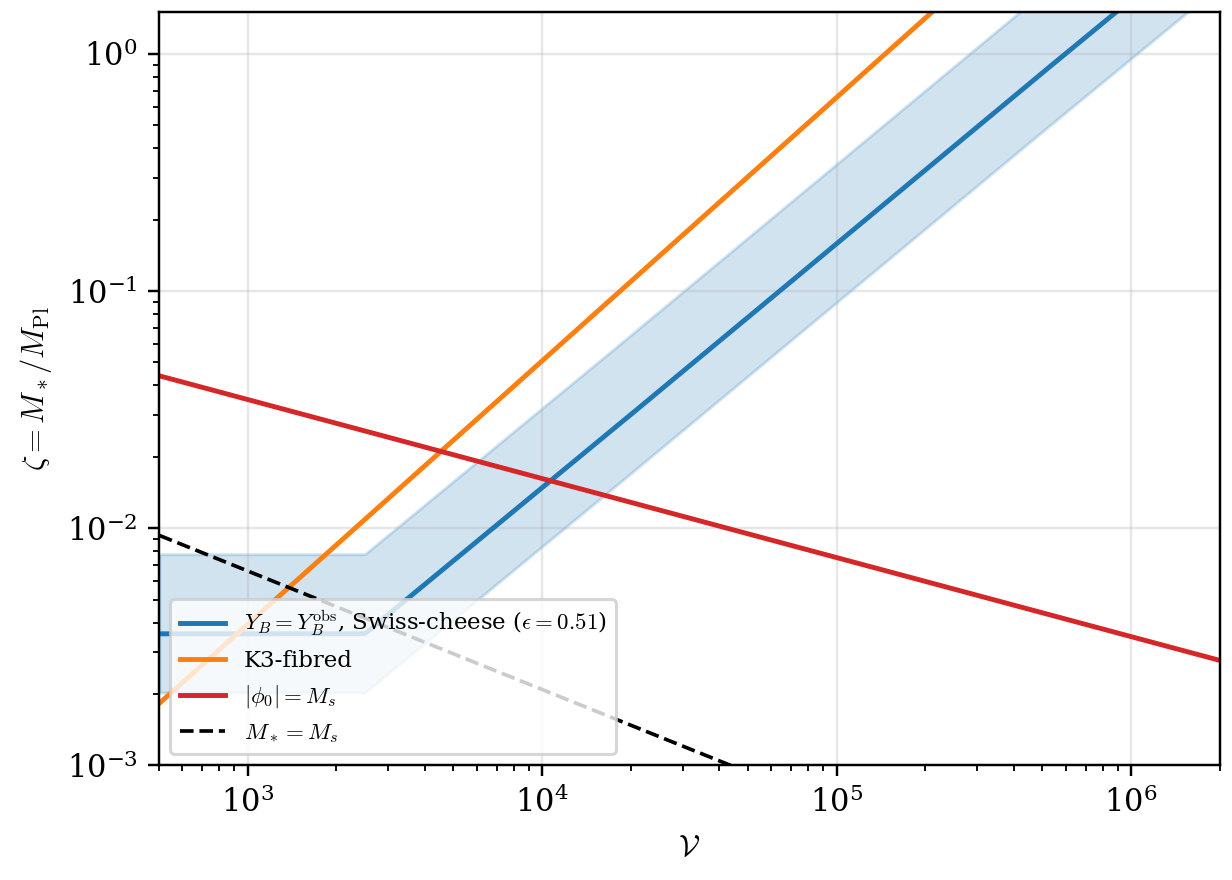
\includegraphics[width=0.6\textwidth]{fig_admap.png}
\caption{Baryonic Affleck--Dine baryogenesis in the plane of volume and operator scale $\zeta=M_*/\Mpl$. The observed asymmetry is reached above the blue line (Swiss-cheese, $\epsilon=0.51$; band: $\epsilon=0.16$--$1.2$) or the orange line (K3-fibred); the effective theory is valid below the red line, $|\phi_0|=M_s$. The dashed line is $M_*=M_s$.}
\label{fig:admap}\end{figure}
The allowed region is shown in Fig.~\ref{fig:admap}. Several further effects bear on the analysis: (i) the blow-up modulus and its axion have $m\simeq(17$--$78)m_{3/2}\gg m_{\rm AD}$, so they begin to oscillate before $H=m_{\rm AD}$ and decay at $H\sim10^4$ GeV, long after, and may dominate the energy density across the epoch in which the flat direction is displaced; Case~I assumes inflaton-driven expansion. (ii) The condensate can fragment into Q-balls; this changes the dynamics but not the total charge. (iii) With $m_{\rm AD}\gtrsim10^9$ GeV the low-energy theory is not supersymmetric and dark matter must be supplied separately. (iv) The sequestered case is more favourable, since $|\phi_0|\propto m_{\rm AD}^{1/4}$, but the analysis of Hubble-induced terms during modulus domination is beyond the scope of this paper.

The conclusion is that baryonic Affleck--Dine baryogenesis with gravity-mediated soft terms does not give a controlled window in LVS at large volume; it is possible at $\vol\lesssim10^4$ (K3: $5\times10^3$) or with sequestered soft terms. Affleck--Dine baryogenesis in LVS was studied in \cite{HKT1}; the present analysis concerns the case in which the modulus itself dilutes the asymmetry, as in \cite{KN}.

\section{Discussion}

Within the assumptions stated (a single modulus-dominated era, no thermal inflation), electroweak-scale baryogenesis before the decay, axion-velocity mechanisms with bulk, fibre or blow-up axions, and leptogenesis from modulus decay are excluded in LVS at the volumes that give TeV-scale supersymmetry. What remains is baryon-violating decay, which for sequestered soft terms and TeV-scale superpartners at $\vol\sim10^7$--$10^8$ requires $\epsilon\sim10^{-4}$--$10^{-3}$, through the Higgs and higgsino channels since the gaugino channel is closed, where the gluino-loop asymmetry vanishes for a pure higgsino and reaches the required size only for a bino admixture of at least $25\%$, and Affleck--Dine baryogenesis, whose controlled regime is small volume or sequestered soft terms. The sphaleron results of Sec.~\ref{sec:sph} apply to any modulus-dominated cosmology, and the required baryon number per decay, $\epsilon\sim10^{-4}$--$10^{-3}$, is common to the IIB, heterotic, $G_2$ and LVS constructions (Table~\ref{tab:cross}).

\paragraph*{Limitations.} (1) The lattice parametrisation is discontinuous at $T_c$ and $c$ is calibrated; efficiencies are uncertain at $O(1)$ through $c$, though the exponent in $\eta_L\propto T_R^4$ is robust. (2) $g_*(T)$ is approximated near the QCD crossover. (3) The Swiss-cheese vacua are AdS and use $W_0=A=1$; $c_\Gamma$ is a parameter, and varying it over $[0.3,8]$ changes $\vol_{\max}$ by a factor $\lesssim2$. (4) The K3 loop potential is conjectural \cite{CBQ}; variations in the loop data change $\vol_{\max}$ by a factor $\lesssim4$. (5) All bounds assume the lightest modulus dominates (Sec.~\ref{sec:emde}) and, for $T_R\lesssim1$ GeV, a specific pre-oscillation history. (6) The kinetic bound assumes Chern--Simons-driven baryogenesis; non-sphaleron axion mechanisms are not constrained. (7) $\epsilon$ for baryon-violating decays and the string-theoretic origin of the $A$-terms are not derived.

\paragraph*{Data and code.} All numerical results are generated by the code at \url{https://github.com/vishal1601-2005/Entropy-walls-LVS} (MIT licence), which contains the intermediate data and the \LaTeX\ source. The inputs are the lattice rate \cite{DRT14}, the K3 parameter sets \cite{CBQ} and $Y_B^{\rm obs}$.

\appendix
\section{Dilution coefficient}
Let the sudden-decay entropy be $S_{\rm fin}=\tfrac{2\pi^2}{45}g_RT_R^3a_d^3$, with $\rho_\phi(a_d)=3\Mpl^2\Gamma^2$. Since $\rho_\phi\propto H^2$ and $\rho_\phi\propto a^{-3}$, $a_d^3/a_{\rm gen}^3=H_{\rm gen}^2/\Gamma^2$, with $H_{\rm gen}$ from Eq.~(\ref{eq:Hss}). Hence
\begin{equation}
\mathcal D=\frac{g_*}{g_R}\Big(\frac{T_{\rm gen}}{T_R}\Big)^3\Big(\frac{\Gamma}{H_{\rm gen}}\Big)^2,\qquad
\frac{\Gamma}{H_{\rm gen}}=\frac{b}{\kappa}\Big(\frac{T_R}{T_{\rm gen}}\Big)^4,\qquad \frac b\kappa=\frac{36\,b^2}{\pi^2g_*}=0.4\,\frac{g_R}{g_*},
\end{equation}
with $b=\sqrt{\pi^2g_R/90}$. Therefore $\mathcal D=0.16\,(g_R/g_*)(T_R/T_{\rm gen})^5$, which is Eq.~(\ref{eq:D}). The same ratio gives $\Gamma/H(T)=\tfrac{2g_R}{5g_*}(T_R/T)^4$ used in Sec.~\ref{sec:boltz}.

\section{Susceptibility}
In units of $T^2/6$ per species, with flavour-universal potentials, hypercharge neutrality reads $n_g[\mu_Q+2\mu_u-\mu_d-\mu_L-\mu_e]+2\mu_H=0$ (the Higgs term carries the bosonic factor). With $\mu_u=\mu_Q+\mu_H$, etc., this gives $\mu_H=\tfrac37(\mu_L-\mu_Q)$. Then $B=12\mu_Q$, $B-L=12\mu_Q-9\mu_L+3\mu_H$, and $\mu_{\rm CS}=9\mu_Q+3\mu_L$. For $B-L=0$, $\mu_L=\tfrac{25}{18}\mu_Q$ and $\mu_Q=\tfrac{6}{79}\mu_{\rm CS}$, so $n_B=\tfrac{12}{79}T^2\mu_{\rm CS}$. For $\mu_{\rm CS}=0$, $\mu_L=-3\mu_Q$ and $B/(B-L)=28/79$.

\section{K\"ahler metric of the blow-up modulus}
For $K=-2\ln\vol$ with $\vol=\gamma(\tau_b^{3/2}-\tau_s^{3/2})$ and $\tau=\tfrac12(T+\bar T)$, $K_{s\bar s}=\tfrac14\partial_{\tau_s}^2K$. For $\tau_s^{3/2}\ll\tau_b^{3/2}$, $K=-2\ln(\gamma\tau_b^{3/2})+2\tau_s^{3/2}/\tau_b^{3/2}+\dots$, hence $K_{s\bar s}\simeq3\gamma/8\sqrt{\tau_s}\vol$. We checked this against the exact second derivative at $\vol=1.5\times10^{14}$, $\tau_s=25.1$ (four digits).


\section{Explicit amplitude check of the CP asymmetry}\label{app:amp}
With the stops integrated out, the interactions are
\begin{equation}
\mathcal L_{\rm eff}=\sum_{\alpha\beta}D_{\alpha\beta}\,J_\alpha^*J_\beta,\qquad
J_\alpha=\sum_{i=1,2}\Big[A_{i\alpha}(\lambda_i\psi_Q)+B_{i\alpha}(\lambda_i^\dagger\psi_{U^c}^\dagger)\Big]+\delta_{\alpha R}\,\rho\,(\psi_{b^c}\psi_{s^c}),
\end{equation}
with $\alpha\in\{R,L\}$, $D=(M^2_{\tilde t})^{-1}$, and $\lambda_{1,2}$ the Majorana fermions. For the gluino $A_L=-\sqrt2g_3$, $B_R=\sqrt2g_3$; for the neutral higgsino $A_R=B_L=-y_t/\sqrt2$; for a bino admixture $B_R=\tfrac{2\sqrt2}{3}g_1a_B$ and $A_L=-\tfrac{\sqrt2}{6}g_1a_B$. The tree amplitudes for $\lambda_1\to tsb$ and $\bar t\bar s\bar b$, the three-body amplitude for $\lambda_1\to t\lambda_2\bar t$ (two diagrams, since $\lambda_2$ is Majorana) and the amplitude for $\lambda_2\bar t\to bs$ are evaluated with explicit two-component spinors. The absorptive part follows from unitarity,
\begin{equation}
\mathcal T^{\rm abs}_{fi}=\tfrac{i}{2}\sum_n\int d\Phi_n\,\mathcal T_{fn}\mathcal T_{ni},\qquad n=(\lambda_2,t,\bar t),
\end{equation}
with the top a spectator, and the asymmetry is $\Gamma(f)-\Gamma(\bar f)$ integrated over the three-body phase space. The relative sign of the $f$ and $\bar f$ cuts is a fermion-ordering sign; with the opposite sign the asymmetry vanishes identically, and the sign used reproduces \cite{KW} for right-handed couplings.

The implementation reproduces the tree rate (39) of \cite{KW} for all stop mixings and couplings tested, and the cross-chirality terms of (40). For right-handed couplings it reproduces the $f_2$ term of (41), with the dependence on $x=m_{\tilde\lambda_2}^2/m_{\tilde\lambda_1}^2$ confirmed at $x=0.09,\,0.25,\,0.49$ and the dependence $\sin\phi_{12}$ on the phase. It differs from (41) in two respects. First, the left-handed term $\kappa_{1L}^2\kappa_{2L}^2c_t^2s_t^4$ enters with the opposite sign to the right-handed one. Second, there is no $f_1$ term. Both follow from rephasing invariance: a term without a gaugino mass insertion cannot depend on the phase of the gaugino mass, and the right- and left-handed mass-insertion terms carry opposite phases. The same-chirality three-body rate differs from (40) by $3\%$ at $x=0.25$. Neither difference affects the right-handed benchmark (47).

\begin{thebibliography}{99}
\bibitem{Coughlan}G.~D.~Coughlan \emph{et al.}, Phys.\ Lett.\ B \textbf{131}, 59 (1983).
\bibitem{BKN}T.~Banks, D.~B.~Kaplan, A.~E.~Nelson, Phys.\ Rev.\ D \textbf{49}, 779 (1994), hep-ph/9308292.
\bibitem{dCCQR}B.~de Carlos, J.~A.~Casas, F.~Quevedo, E.~Roulet, Phys.\ Lett.\ B \textbf{318}, 447 (1993), hep-ph/9308325.
\bibitem{BBCQ}V.~Balasubramanian, P.~Berglund, J.~P.~Conlon, F.~Quevedo, JHEP \textbf{03} (2005) 007, hep-th/0502058.
\bibitem{CQS}J.~P.~Conlon, F.~Quevedo, K.~Suruliz, JHEP \textbf{08} (2005) 007, hep-th/0505076.
\bibitem{CPS}K.~Choi, W.-I.~Park, C.~S.~Shin, JCAP \textbf{03} (2013) 011, arXiv:1211.3755.
\bibitem{CCQ}M.~Cicoli, J.~P.~Conlon, F.~Quevedo, Phys.\ Rev.\ D \textbf{87}, 043520 (2013), arXiv:1208.3562.
\bibitem{HT}T.~Higaki, F.~Takahashi, JHEP \textbf{11} (2012) 125, arXiv:1208.3563.
\bibitem{CBQ}M.~Cicoli, C.~P.~Burgess, F.~Quevedo, JCAP \textbf{03} (2009) 013, arXiv:0808.0691.
\bibitem{DLR}S.~Davidson, M.~Losada, A.~Riotto, Phys.\ Rev.\ Lett.\ \textbf{84}, 4284 (2000), hep-ph/0001301.
\bibitem{Garcia}M.~A.~G.~Garcia, S.~E.~Henrich, W.~Ke, K.~A.~Olive, ``Leptogenesis and low reheating temperatures,'' arXiv:2607.08663.
\bibitem{McDonald}J.~McDonald, Phys.\ Rev.\ D \textbf{43}, 1063 (1991).
\bibitem{GKR}G.~F.~Giudice, E.~W.~Kolb, A.~Riotto, Phys.\ Rev.\ D \textbf{64}, 023508 (2001), hep-ph/0005123.
\bibitem{CoHarigaya}R.~T.~Co, K.~Harigaya, Phys.\ Rev.\ Lett.\ \textbf{124}, 111602 (2020), arXiv:1910.02080.
\bibitem{Snowmass}``New Ideas in Baryogenesis: A Snowmass White Paper,'' arXiv:2203.05010.
\bibitem{Asadi}P.~Asadi, D.~Cyncynates, S.~Gori, ``Axiverse baryogenesis,'' arXiv:2511.15794.
\bibitem{BCKMQ}R.~Blumenhagen, J.~P.~Conlon, S.~Krippendorf, S.~Moster, F.~Quevedo, JHEP \textbf{09} (2009) 007, arXiv:0906.3297.
\bibitem{DRT14}M.~D'Onofrio, K.~Rummukainen, A.~Tranberg, Phys.\ Rev.\ Lett.\ \textbf{113}, 141602 (2014), arXiv:1404.3565.
\bibitem{KN}M.~Kawasaki, K.~Nakayama, ``Baryon asymmetry in heavy moduli scenario,'' arXiv:0705.0079.
\bibitem{HKT1}T.~Higaki, K.~Kamada, F.~Takahashi, ``Higgs, moduli problem, baryogenesis and large volume compactifications,'' arXiv:1207.2771.
\bibitem{IJT}K.~Ishiwata, K.~S.~Jeong, F.~Takahashi, ``Moduli-induced baryogenesis,'' JHEP \textbf{02} (2014) 062, arXiv:1312.0954.
\bibitem{KW}G.~Kane, M.~W.~Winkler, ``Baryogenesis from a modulus dominated universe,'' arXiv:1909.04705.
\bibitem{Haghi}B.~Shams Es Haghi, ``Baryogenesis and primordial black hole dark matter from heavy metastable particles,'' arXiv:2212.11308.
\end{thebibliography}
\end{document}
